\documentclass{article}
\usepackage[preprint,nonatbib]{neurips_2026}
\usepackage[T1]{fontenc}
\usepackage[utf8]{inputenc}
\usepackage{amsmath,amssymb,booktabs,graphicx,microtype,xcolor}
\usepackage[colorlinks=true,allcolors=linkblue]{hyperref}
\definecolor{linkblue}{HTML}{1849A9}
\hypersetup{pdftitle={Can a neural network learn the remainder?},pdfauthor={Antreas Antoniou},pdfsubject={Modulo 7: completed small-data screen and preliminary million-example validation}}
\newcommand{\repo}{https://github.com/AntreasAntoniou/learning-modulo-seven}
\newcommand{\smallnote}[1]{{\small\color{black!70}#1}}
\title{Can a neural network learn the remainder?\\
\large Modulo 7, data scale, and generalisation beyond the training range}
\author{Antreas Antoniou\\
\href{https://antreas.io}{antreas.io} \quad $\cdot$ \quad \href{\repo}{Code, measurements and editable report}}
\begin{document}
\maketitle
\begin{center}
\small\textbf{Working research report $\cdot$ 14 October 2026 $\cdot$ Version 0.1}\\
Completed small-data screen; preliminary validation from the million-example follow-up.\\
Independent report using the NeurIPS preprint template; not a NeurIPS submission.
\end{center}

\begin{abstract}
Modulo 7 is a tiny program and an awkward learning problem. Adjacent integers usually
have different labels, yet the answer repeats forever. I wanted to see what happens
when we ask ordinary neural architectures to discover that structure from examples,
and how the answer changes with representation, depth and data. We compare scalar
and binary inputs across 16 architecture variants and three training-set sizes.
In the completed screen, a shallow conditional hypernetwork reaches
\textbf{94.56\% $\pm$ 2.12\%} on unseen integers within the training range with
65,536 examples, but \textbf{11.94\% $\pm$ 2.39\%} outside it. Smaller datasets leave
that configuration near chance. Other hypernetworks sometimes succeed with 4,096
examples, with substantial variation across seeds. A separate diagnostic exposing
every bit during training improves some outside-range outcomes without making them
reliable. We then specify a larger, ongoing experiment: one million unique examples,
ten passes, three weight decays and three seeds. Its first twelve completed fits
already show that very accurate within-range validation can coexist with widely
different outside-range behaviour. Final model selection and test evaluation for
that sweep have not happened. Throughout, $\pm$ denotes sample standard deviation
over three optimisation seeds, not a confidence interval.
\end{abstract}

\section{A small function with a useful sting}
Take an integer, divide by seven, keep the remainder. The labels are
$0,1,2,3,4,5,6,0,1,\ldots$. There is almost nothing to the program. But if all we give
a network is a collection of input--output pairs, the useful structure has to come
from somewhere: the input representation, the architecture, or what optimisation
manages to build out of the examples.

This is what I wanted to poke at. A model can be quite good at filling gaps between
the numbers it has seen and still have no dependable way to continue the pattern.
So we ask two separate questions. Can it predict \emph{unseen values within the
training range}? And does that prediction survive when we move \emph{outside the
range}? Calling both of those ``generalisation'' and reporting one number would
throw away much of what makes this experiment interesting.

The original screen also included sphere volume, multiplication, a chirp and a
pairwise-distance task. Sphere volume is a smooth cubic control, so ``nonlinear''
should not be mistaken for ``intrinsically difficult.'' A fitted cubic solves that
control to numerical precision. This report concentrates on modulo, where the
representation and data-size effects were particularly clear. The repository
retains the complete measurements for the other tasks too.

\newpage
\section{What the models actually receive}
The target is a seven-way classification problem, $y=n\bmod 7$, trained with
cross-entropy. We use two encodings of the same integers. The scalar version maps
the within-range interval to $[-1,1]$. The binary version supplies each bit as
$-1$ or $+1$. Neither supplies the remainder or hand-designed periodic features.

These are very different starting points. In the scalar representation, moving
one integer along the line usually changes the answer. In binary, the bits expose
a compositional route to the answer. If $n=\sum_k b_k2^k$, then
\[
 n\bmod 7=\left(\sum_k b_k(2^k\bmod 7)\right)\bmod 7,
 \qquad 2^k\bmod 7=1,2,4,1,2,4,\ldots.
\]
That identity explains an available structure; we do not build it into the learned
models. The exact modulo operation is the label oracle, not a learned baseline.

\subsection{Architecture is more than the number of layers}
The plain MLPs have 3, 20 or 50 linear layers, including the output, with GELU
between hidden layers. Residual 20- and 50-layer MLPs provide a control for making
depth trainable. Transformer variants have 2, 8 or 12 pre-normalised blocks, four
attention heads, a learned position for each numeric feature and a classification
token. Each bit becomes a token; scalar input gives just one numeric token.

The relational variants take 2, 8 or 12 rounds of pairwise messages. A learned
two-layer function processes every ordered pair, including self-pairs; messages
are averaged and added to the receiving representation. Each round has its own
parameters. This is a small adaptation of the relational-network idea
\cite{relational}, not a replication of its original experiments. A scalar input
gives this module very little relational structure to work with.

The conditional hypernetworks have the form the experiment was designed to test:
\[
  \hat y=f(x,w),\qquad w=g(x;\theta).
\]
Only $\theta$ is independently learned. For each example, $g$ emits \emph{all}
weights and biases of $f$; $f$ then processes that same example. Gradients pass
through both computations, but $f$ owns no stored trainable parameters. The idea
of generating one network's weights with another goes back to HyperNetworks
\cite{hyper}; here the generation is conditioned directly on the current input.
We vary $g$'s depth over 2, 8 and 12 at $f$ depth 3, then vary $f$ over 1, 3 and 5
at $g$ depth 8. Hidden layers in $f$ have width eight.

Widths are chosen to approach 32,768 learned parameters. That makes deeper models
narrower. It also leaves discrete differences in parameter count, especially for
four-head transformers. Generated coefficients are counted separately from learned
parameters. We are comparing small models with roughly matched parameter counts;
we are not matching FLOPs or claiming every architecture receives its best recipe.

\subsection{The completed screen}
We use 256, 4,096 and 65,536 nested training examples, seeds 101/202/303, and learning
rates $3\times10^{-4}$ and $3\times10^{-3}$. AdamW \cite{adamw} uses zero weight
decay, default $\beta=(0.9,0.999)$ and $\epsilon=10^{-8}$, no dropout, gradient-norm
clipping at one, and batch size 128. Every fit receives 1,200 optimiser steps with
sampling \emph{with replacement}: 153,600 example presentations. Validation is
recorded at step one and every 100 steps. Checkpoints and learning rates are chosen
using within-range validation loss alone, separately for each seed. Test metrics
are recorded for each fit's selected checkpoint; they do not choose its checkpoint
or learning rate. The million-example follow-up uses a stricter delayed test phase.

Within-range integers are $[0,131072)$; outside-range integers are $[131072,262144)$.
Each domain has separate validation and test sets of 4,096 and 8,192 values.
All five splits are disjoint. The data seed is fixed at 1729, so the three reported
seeds measure optimisation variability on one dataset, not variability across
independently sampled datasets.

\newpage
\section{More data changes the answer, but not monotonically}
\begin{figure}[h!]
\centering
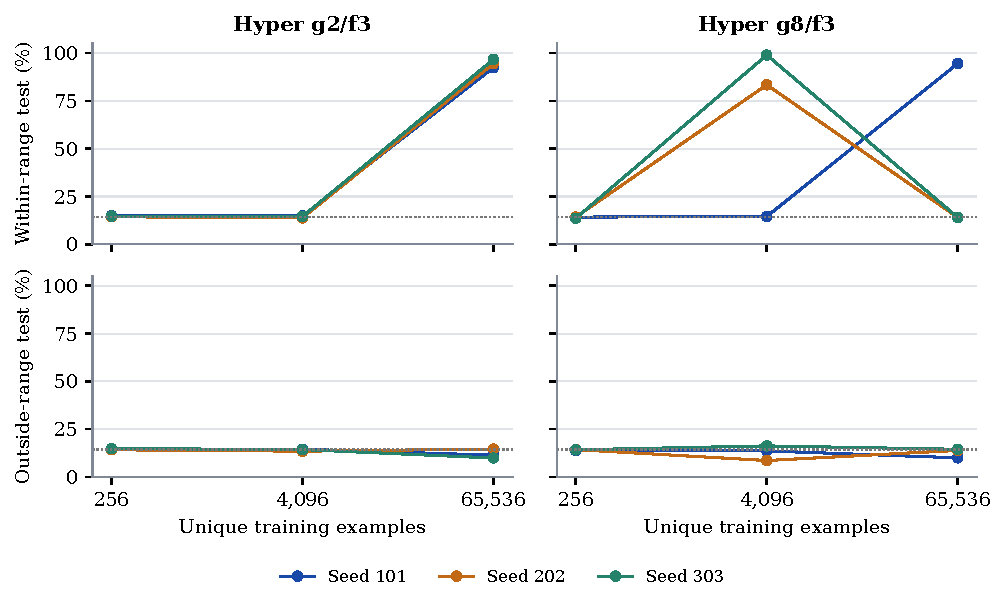
\includegraphics[width=\linewidth]{figures/data-and-seeds.pdf}
\caption{Completed primary screen. Each line is one optimisation seed; the two
learning rates are selected by within-range validation for that seed. Dotted lines
mark uniform chance, $1/7$. Training steps are fixed across data amounts. Points
at different amounts are separate fits, not a continuation of one model.}
\label{fig:scale}
\end{figure}

For the shallow $g2/f3$ hypernetwork, increasing the pool to 65,536 examples produces
a result that repeats across all three seeds: 92.44\%, 94.56\% and 96.69\% within-range
test accuracy. At 256 and 4,096 examples, its mean accuracy is 14.68\% and 14.40\%.
There is a large change here, and three good seeds are much more useful evidence
than the most flattering single run.

But the next hypernetwork makes the story less tidy. For $g8/f3$, 4,096 examples
produce 14.56\%, 83.42\% and 99.01\%; 65,536 produce 94.54\%, 14.06\% and 14.03\%.
So 4,096 can be enough for a successful fit. It was not reliably enough under this
recipe, and adding data did not reliably rescue this deeper generator either.

There is an important budget detail behind the figure. Keeping 1,200 steps fixed
means the nominal exposure is 600, 37.5 or 2.34375 passes through the three pools.
The largest-pool runs encounter approximately 59,300 distinct training values over
the full run, rather than every one of the 65,536. A selected checkpoint may be
earlier still. We therefore cannot read this as a clean estimate of what data
alone buys after each model has fully converged.

Scalar-input modulo stays near chance throughout the tested screen. Most binary
architectures do too (Appendix~\ref{sec:full}). This says something about these
representations and recipes. It does not say that MLPs, transformers or relational
networks are incapable of modular arithmetic. The plain 50-layer MLP also struggles
on the smooth controls, while residual connections restore substantial learning.
Making a stack deeper changes optimisation as well as its representational capacity.

\newpage
\section{The outside-range problem is doing real work}
The successful shallow hypernetwork's 94.56\% within-range score becomes
11.94\% outside the range. That is below uniform chance on this particular held-out
sample. A network that has learnt the general modular rule should not care that
the integer is larger. Something in the fitted computation does.

There is a specific complication in the primary binary split: the eighteenth bit
is always zero during training and always one outside. The model is being asked to
handle a previously unseen feature value. To explore that issue we ran a separate
diagnostic with 17 bits, training within $[0,98304)$ and evaluating outside on
$[98304,131072)$. Every individual bit now varies during training. What remains
unseen is the joint top-two-bit combination $11$.

\begin{table}[h!]
\centering
\caption{Shallow hypernetwork $g2/f3$, 65,536 training examples. Test accuracy
(percent), mean $\pm$ sample SD over three seeds. The diagnostic was declared after
inspection of the first primary seed and is reported separately.}
\small
\begin{tabular}{lrr}
\toprule
Domain design & Within range & Outside range\\
\midrule
Primary: new high-bit value outside & $94.56\pm2.12$ & $11.94\pm2.39$\\
Diagnostic: familiar bits, new joint pattern & $81.40\pm11.27$ & $36.68\pm28.79$\\
\bottomrule
\end{tabular}
\end{table}

The three diagnostic outside scores are 13.21\%, 28.04\% and 68.80\%. There is
useful extrapolation in some fits, but the variability is too large to call the
behaviour dependable. And the diagnostic changes the range, bit width, data stream
and training fraction together. It cannot isolate the causal contribution of
exposing the high bit. We should resist giving it that job after the fact.

\subsection{Is the hypernetwork taking a shortcut through a bias?}
There is an obvious question about $f(x,g(x;\theta))$. Since the generator sees the
input, perhaps it simply predicts the answer in the generated output bias and
the rest of $f$ is decorative. A frozen decomposition gives a useful first check.
On the primary binary task at 65,536 examples, $g2/f3$ scores 14.73\% $\pm$ 1.99\%
using only its final generated bias, compared with 94.56\% $\pm$ 2.12\% as the full
model. Subtracting that bias from the full prediction leaves 90.69\% $\pm$ 3.24\%.

The final bias alone is not carrying the successful prediction. That is as far as
this probe gets us. Other generated coefficients can carry input-dependent
information, and removing a component after joint training is different from
retraining without it. We have not identified a modular algorithm inside the
network, or shown that a particular depth of $f$ is necessary.

\subsection{A note on the smooth controls}
The broader screen helps keep the interpretation grounded. With 65,536 examples,
a $g8/f1$ hypernetwork achieves outside-range $R^2=0.99626$ on multiplication and
$0.93341$ on sphere volume, averaged over seeds. Good extrapolation is possible
on these finite domains. The chirp behaves very differently: some accurate
within-range models produce very large outside errors. Whether a model fits a
function and how it continues beyond the observations remain separate empirical
questions, even before we get to modulo.

\newpage
\section{The million-example experiment}
The follow-up keeps the full architecture comparison, expands the integer range,
and gives every fit ten complete shuffled passes through one million unique
training values. This is a different regime from the short screen. It changes
range, exposure, bit width and regularisation together; it is not another point
on Figure~\ref{fig:scale}'s data-size axis.

\begin{table}[h!]
\centering
\caption{Frozen follow-up design. Intervals are half-open. Validation and test
values are disjoint from training and from one another.}
\small
\begin{tabular}{p{2.0in}p{3.0in}}
\toprule
Item & Setting\\
\midrule
Within-range domain & $[0,3145728)$\\
Outside-range domain & $[3145728,4194304)$\\
Training / validation / test & 1,000,000 training; 8,192 validation and 65,536 test per domain\\
Representation & Scalar and 22 binary features; every training bit varies\\
Grid & 16 variants $\times$ 2 encodings $\times$ 2 learning rates $\times$ 3 decays $\times$ 3 seeds = 576 fits\\
Learning rates / weight decay & $0.0003,0.003$ / $0,0.01,0.1$\\
Optimisation & AdamW; $\beta=(0.9,0.999)$; $\epsilon=10^{-8}$; constant learning rate\\
Other settings & Dropout 0; norm clipping 1; float32; TF32 disabled; decay applied to all learned parameters, including biases and normalisation\\
Exposure per fit & 10 passes; 10,000,000 presentations; 80,000 updates\\
Logging & Every training batch; both validation domains every 5,000 presentations\\
\bottomrule
\end{tabular}
\end{table}

The batch size is 128, with one small adjustment: $5000=39\times128+8$. Each
validation boundary therefore finishes with an eight-example batch. This gives
exactly the requested cadence without skipping or duplicating examples. Training
loss in the figures is the example-weighted mean over those 5,000 presentations,
not an unweighted mean that would give the eight-example batch disproportionate
influence. Each fit has 2,000 validation observations.

Both validation sets are monitored, but \textbf{only within-range validation selects
models}. Each fit retains the checkpoint with the lowest within-validation
cross-entropy, using accuracy to break an exact tie and the earlier checkpoint
if both tie. Once all 576 fits finish, we choose a learning-rate/weight-decay pair
for each architecture and encoding by the mean best validation loss across its
three seeds. We retain all three seeds of that configuration. An overall
validation winner is also recorded for each encoding.

Only after those choices are frozen will the 96 retained models enter the single
final test phase, on both held-out domains. The training worker receives no test
file. The test evaluator uses a create-once execution record, and the selector
rejects incomplete or mismatched sweeps. These controls protect the procedure;
they do not make repeated validation observations independent evidence.

The outside range again holds out the top-two-bit pattern $11$, while $00$, $01$
and $10$ occur within range. This probes a new combination at fixed bit length.
Even perfect performance here would not establish generalisation to arbitrary
integer lengths or to every larger number.

\newpage
\section{First completed trajectories: encouraging, uneven, still validation}
\begin{figure}[h!]
\centering
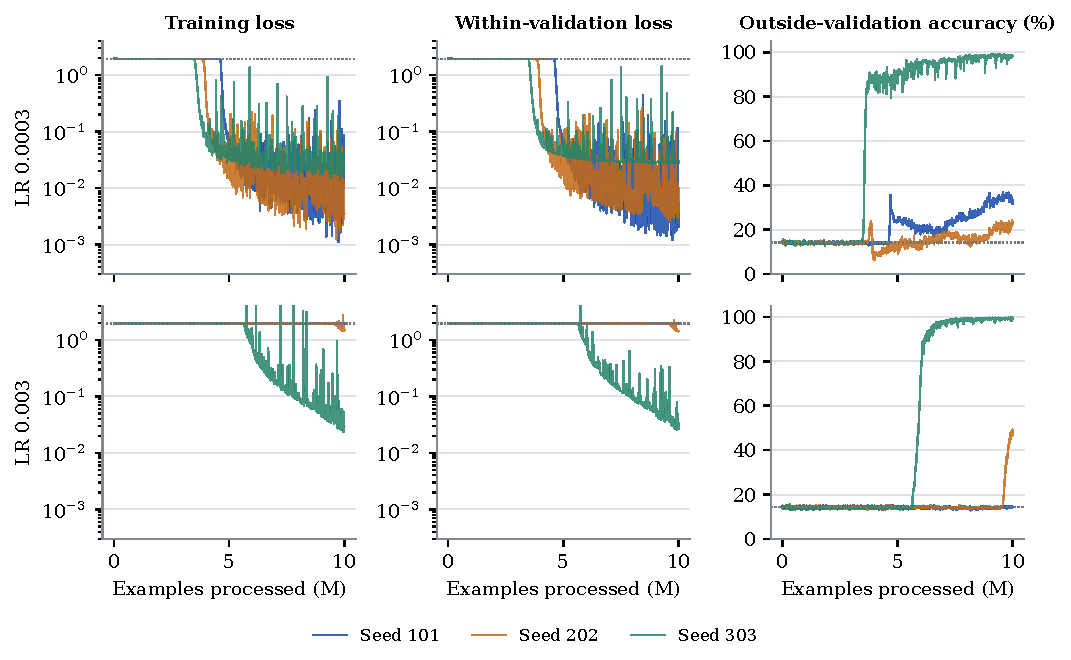
\includegraphics[width=\linewidth]{figures/million-learning-curves.pdf}
\caption{The first six completed zero-decay fits of binary $g2/f3$, through ten
million presentations. Training loss is averaged over exact 5,000-example windows;
both loss axes are logarithmic. Outside accuracy uses the diagnostic validation
set. Dotted lines mark uniform-prediction cross-entropy $\log 7$ or accuracy $1/7$.
These are six fits from an ongoing 576-fit sweep, not a comparison of all families.}
\label{fig:live}
\end{figure}

At the lower learning rate, all three zero-decay seeds reach more than 99\%
within-range validation accuracy at their selected checkpoint. Yet their
outside-validation accuracies are 35.16\%, 19.01\% and 98.23\%. The same
architecture, dataset and optimiser can arrive at solutions that agree almost
perfectly on the familiar range and behave very differently beyond it.

The higher learning rate makes the seed sensitivity even harder to ignore. One
zero-decay seed reaches 99.88\% within and 99.72\% outside validation; another
remains near chance at its selected checkpoint. That successful seed is worth
investigating. It is not a reliable three-seed result.

The curves also stop us from naming every late improvement ``grokking.'' In the
classic usage, generalisation improves long after training performance has become
good \cite{grokking}. In the lower-learning-rate trajectories here, training and
within-validation loss improve together during a late sharp change. We have not
established a prolonged memorisation-then-generalisation separation.

This public snapshot includes \textbf{twelve completed fits}, collected on
\textbf{14 October 2026 at 13:06 UTC}: $g2/f3$ only, two learning rates, weight decays
0 and 0.01, all three seeds. Weight decay 0.1 and the remaining architecture grid
are absent from this frozen snapshot. The next page lists every included outcome,
including the failures. No weight-decay winner has been chosen, and no test
evaluation has been performed for the million-example experiment.

\newpage
\begin{table}[t!]
\centering
\caption{Every completed million-example fit in this snapshot. All rows are
binary $g2/f3$. The checkpoint is selected by within-validation cross-entropy.
Outside accuracy is measured at that same checkpoint, not at its own maximum.
The checkpoint column counts millions of example presentations.}
\small
\begin{tabular}{rrrrrrr}
\toprule
Decay & LR & Seed & Checkpoint & Within CE & Within (\%) & Outside (\%)\\
\midrule
0 & 0.0003 & 101 & 9.750 & 0.0012 & 99.98 & 35.16 \\
0 & 0.0003 & 202 & 9.640 & 0.0027 & 99.91 & 19.01 \\
0 & 0.0003 & 303 & 10.000 & 0.0279 & 99.37 & 98.23 \\
0 & 0.003 & 101 & 5.145 & 1.9453 & 15.44 & 14.04 \\
0 & 0.003 & 202 & 10.000 & 1.4278 & 34.75 & 48.55 \\
0 & 0.003 & 303 & 9.935 & 0.0260 & 99.88 & 99.72 \\
0.01 & 0.0003 & 101 & 9.915 & 0.0032 & 99.93 & 39.48 \\
0.01 & 0.0003 & 202 & 9.935 & 0.0068 & 99.78 & 91.10 \\
0.01 & 0.0003 & 303 & 9.660 & 0.0006 & 99.98 & 96.18 \\
0.01 & 0.003 & 101 & 7.980 & 1.9455 & 14.51 & 13.62 \\
0.01 & 0.003 & 202 & 6.605 & 1.9453 & 14.86 & 14.22 \\
0.01 & 0.003 & 303 & 8.945 & 1.9457 & 14.88 & 14.36 \\
\bottomrule

\end{tabular}
\label{tab:live}
\end{table}

\section{What I would take from this so far}
Giving a model more examples can change the result dramatically, and starting
with 4,096 examples would have missed the repeatable shallow-hypernetwork result
in the completed screen. At the same time, the deeper generator's mixed seeds
make a simple ``more data fixes it'' conclusion untenable. How the architecture
uses those examples, and where optimisation takes it, matter here.

The most useful tension is between almost perfect prediction inside the domain
and disagreement outside it. That suggests an experiment beyond another
leaderboard: take successful within-range fits, compare the computations they
have acquired, and ask what distinguishes those that extend the rule from those
that do not. Retrained generator/component controls, independent dataset seeds
and carefully matched domain shifts would help answer that. None of those
follow-ups is a result of the current sweep.

For the ongoing experiment, the immediate job is more prosaic: finish the full
grid, keep the bad seeds, freeze the validation choices, and open the test sets
once. If the strongest outside-validation result survives that procedure across
seeds, we will have a much better reason to inspect its mechanism. If it does
not, that will also tell us something useful about how easy it is to mistake one
fortunate training trajectory for a dependable learner.

\paragraph{Scope and limitations.}
The dataset is fixed; three optimisation seeds give limited information about
variability. Architecture widths differ under an approximate parameter budget,
and equal parameters do not mean equal computation. Learning-rate searches are
small. The initial screen is exploratory, and its diagnostic and frozen mechanism
probes were motivated by observed results. The follow-up uses a much longer
training budget and a different domain. Neither experiment tests variable-length
arithmetic, formal algorithm discovery or behaviour over unbounded integers.

\paragraph{Authorship and execution.}
The research question, requested architecture families and follow-up choices are
Antreas's. Protocol development, implementation, analysis and report preparation
were assisted by Codex under his direction. The experiments ran on his Olympus
GPU research infrastructure. This is a working scientific report, not an
independent human review or a peer-reviewed publication.

\newpage
\appendix
\section{All architecture outcomes in the completed screen}\label{sec:full}
\begin{figure}[h!]
\centering
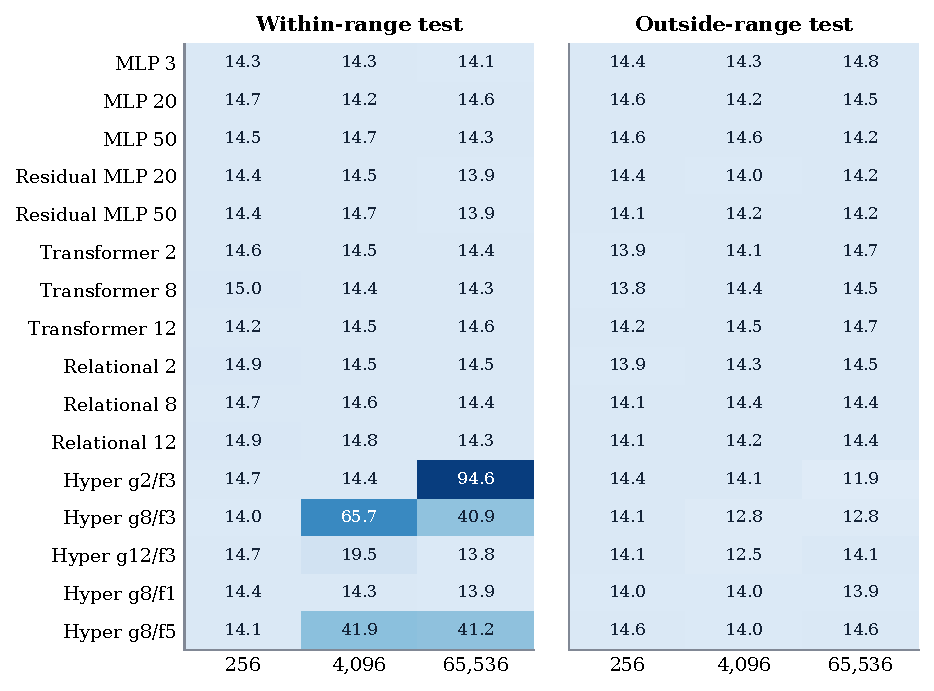
\includegraphics[width=\linewidth]{figures/architecture-grid.pdf}
\caption{Binary modulo 7, all 16 variants and three data amounts. Entries are mean
test accuracy (percent) over the three validation-selected seeds. The underlying
seed rows, standard deviations, losses, validation metrics and both learning-rate
fits are included in the public data. Means can conceal very mixed seed outcomes;
Figure~\ref{fig:scale} shows two examples.}
\end{figure}

\begin{table}[h!]
\centering
\caption{The 65,536-example slice, percent accuracy, mean $\pm$ sample SD.
The scalar outside results are also near chance and are available in the CSV.}
\small
\begin{tabular}{lrrr}
\toprule
Architecture & Scalar within & Binary within & Binary outside\\
\midrule
MLP 3 & 14.45 $\pm$ 0.17 & 14.05 $\pm$ 0.25 & 14.82 $\pm$ 0.13 \\
MLP 20 & 14.55 $\pm$ 0.11 & 14.55 $\pm$ 0.11 & 14.47 $\pm$ 0.33 \\
MLP 50 & 14.34 $\pm$ 0.44 & 14.34 $\pm$ 0.44 & 14.25 $\pm$ 0.36 \\
Residual MLP 20 & 13.98 $\pm$ 0.37 & 13.92 $\pm$ 0.03 & 14.15 $\pm$ 0.22 \\
Residual MLP 50 & 14.25 $\pm$ 0.10 & 13.88 $\pm$ 0.09 & 14.19 $\pm$ 0.25 \\
Transformer 2 & 14.42 $\pm$ 0.11 & 14.43 $\pm$ 0.06 & 14.67 $\pm$ 0.06 \\
Transformer 8 & 14.45 $\pm$ 0.06 & 14.34 $\pm$ 0.24 & 14.48 $\pm$ 0.31 \\
Transformer 12 & 14.63 $\pm$ 0.19 & 14.62 $\pm$ 0.23 & 14.71 $\pm$ 0.09 \\
Relational 2 & 14.22 $\pm$ 0.59 & 14.47 $\pm$ 0.51 & 14.49 $\pm$ 0.33 \\
Relational 8 & 14.47 $\pm$ 0.26 & 14.36 $\pm$ 0.14 & 14.37 $\pm$ 0.30 \\
Relational 12 & 14.29 $\pm$ 0.23 & 14.29 $\pm$ 0.43 & 14.44 $\pm$ 0.15 \\
Hyper g2/f3 & 14.12 $\pm$ 0.33 & 94.56 $\pm$ 2.12 & 11.94 $\pm$ 2.39 \\
Hyper g8/f3 & 14.10 $\pm$ 0.49 & 40.88 $\pm$ 46.48 & 12.76 $\pm$ 2.43 \\
Hyper g12/f3 & 14.14 $\pm$ 0.07 & 13.83 $\pm$ 0.32 & 14.14 $\pm$ 0.50 \\
Hyper g8/f1 & 14.44 $\pm$ 0.34 & 13.91 $\pm$ 0.42 & 13.85 $\pm$ 1.08 \\
Hyper g8/f5 & 14.51 $\pm$ 0.15 & 41.15 $\pm$ 46.79 & 14.58 $\pm$ 0.72 \\
\bottomrule

\end{tabular}
\end{table}

\newpage
\section{Data, checks and reproduction}
\href{\repo}{The public repository} includes all 1,728 primary fits and all 96
diagnostic fits, their recorded learning curves, per-seed selected results and
summary tables. The modulo subset of the primary screen comprises 576 fits.
The million-example snapshot provides its twelve completed fit summaries,
24,000 validation observations and 960,000 individual training-batch records.
Compressed JSONL retains numeric precision; the paper rounds values for readability.

The original completed-screen audit verified 1,840 stored artifacts by exact
generation and SHA-256, recomputed 7,296 evaluation sets, and replayed 912 selected
checkpoints on 16 examples per evaluation split. The replay was a bounded check,
not a full independent retraining. Those archived checkpoint and prediction
payloads are not included in this first public release. Their content hashes are
retained in the exported fit records; the public checks recompute selection and
summary statistics from the released measurements.

For the new snapshot, every checkpoint segment was downloaded with its recorded
generation and verified against its hash. All twelve chains cover presentations
0 through 10,000,000 without gaps. The export checks 80,000 batches and 2,000
validation observations per fit, and independently reconstructs every reported
5,000-example training-loss window. No test file is needed for these checks.
The public protocol suite also checks split separation, scalar encoding uniqueness,
all 32 architecture/encoding forward-and-backward paths, exact sample boundaries,
validation-only selection and deterministic checkpoint resumption on a small CPU
case. These software checks support implementation claims; the scientific results
remain the actual recorded experiments.

\paragraph{Source and environment.}
The repository records source commits and byte hashes for the exported scientific
modules. Primary training used source \texttt{68c142af3f3e}; the observed-bit
diagnostic used \texttt{78d417c1bae3}; the million-example sweep uses
\texttt{de2c10e63431}. The million-example model, data, training and selection files
are exported unchanged. The public version replaces cloud storage with a local
adapter and supplies a local command-line entry point. GPU execution used
PyTorch 2.8.0 with CUDA 12.8, NumPy 2.3.2 and Python 3.13.13; CPU reproduction
can differ numerically from GPU execution.

\paragraph{Resource measurement.}
The completed primary screen and diagnostic consumed 1.62639 allocated GPU-hours,
including setup failures, with one GPU allocated at a time. This measures worker
allocation, not invoiced cost or the longer virtual-machine lifecycle. No final
usage total is yet reported for the ongoing million-example sweep.

\paragraph{Reading the repository.}
Start with \texttt{README.md}; \texttt{PROTOCOL.md} lists the exact splits and
selection rules. \texttt{results/screen/} and \texttt{results/observed\_bits/}
contain completed results. \texttt{results/million/} is explicitly partial.
\texttt{analysis/make\_figures.py} rebuilds the figures and numeric tables from
those files. \texttt{report/report.tex} is the editable report source. The NeurIPS
2026 template is downloaded from its official host in preprint mode, with a pinned
hash; the template does not imply conference affiliation or acceptance.

\begin{thebibliography}{9}
\small
\bibitem{hyper} David Ha, Andrew Dai and Quoc V. Le. \emph{HyperNetworks}. 2016.
\href{https://arxiv.org/abs/1609.09106}{arXiv:1609.09106}.
\bibitem{relational} Adam Santoro, David Raposo, David G. T. Barrett, Mateusz
Malinowski, Razvan Pascanu, Peter Battaglia and Timothy Lillicrap.
\emph{A simple neural network module for relational reasoning}. 2017.
\href{https://arxiv.org/abs/1706.01427}{arXiv:1706.01427}.
\bibitem{adamw} Ilya Loshchilov and Frank Hutter.
\emph{Decoupled Weight Decay Regularization}. 2017.
\href{https://arxiv.org/abs/1711.05101}{arXiv:1711.05101}.
\bibitem{grokking} Alethea Power, Yuri Burda, Harri Edwards, Igor Babuschkin and
Vedant Misra. \emph{Grokking: Generalization Beyond Overfitting on Small Algorithmic
Datasets}. 2022. \href{https://arxiv.org/abs/2201.02177}{arXiv:2201.02177}.
\end{thebibliography}
\end{document}
